%%%%%%%%%%%%%%%%%%%%%%%%%%%%%%%%%%%%%%%%%
% Beamer Presentation
% LaTeX Template
% Version 1.0 (10/11/12)
%
% This template has been downloaded from:
% http://www.LaTeXTemplates.com
%
% License:
% CC BY-NC-SA 3.0 (http://creativecommons.org/licenses/by-nc-sa/3.0/)
%
%%%%%%%%%%%%%%%%%%%%%%%%%%%%%%%%%%%%%%%%%

%----------------------------------------------------------------------------------------
%	PACKAGES AND THEMES
%----------------------------------------------------------------------------------------

\documentclass[handout]{beamer}

\mode<presentation> {

% The Beamer class comes with a number of default slide themes
% which change the colors and layouts of slides. Below this is a list
% of all the themes, uncomment each in turn to see what they look like.

%\usetheme{default}
%\usetheme{AnnArbor}
%\usetheme{Antibes}
%\usetheme{Bergen}
%\usetheme{Berkeley}
%\usetheme{Berlin}
%\usetheme{Boadilla}
%\usetheme{CambridgeUS}
%\usetheme{Copenhagen}
%\usetheme{Darmstadt}
%\usetheme{Dresden}
%\usetheme{Frankfurt}
%\usetheme{Goettingen}
%\usetheme{Hannover}
%\usetheme{Ilmenau}
%\usetheme{JuanLesPins}
%\usetheme{Luebeck}
\usetheme{Madrid}
%\usetheme{Malmoe}
%\usetheme{Marburg}
%\usetheme{Montpellier}
%\usetheme{PaloAlto}
%\usetheme{Pittsburgh}
%\usetheme{Rochester}
%\usetheme{Singapore}
%\usetheme{Szeged}
%\usetheme{Warsaw}

% As well as themes, the Beamer class has a number of color themes
% for any slide theme. Uncomment each of these in turn to see how it
% changes the colors of your current slide theme.

%\usecolortheme{albatross}
%\usecolortheme{beaver}
%\usecolortheme{beetle}
%\usecolortheme{crane}
%\usecolortheme{dolphin}
%\usecolortheme{dove}
%\usecolortheme{fly}
%\usecolortheme{lily}
%\usecolortheme{orchid}
%\usecolortheme{rose}
%\usecolortheme{seagull}
%\usecolortheme{seahorse}
%\usecolortheme{whale}
%\usecolortheme{wolverine}

%\setbeamertemplate{footline} % To remove the footer line in all slides uncomment this line
%\setbeamertemplate{footline}[page number] % To replace the footer line in all slides with a simple slide count uncomment this line

%\setbeamertemplate{navigation symbols}{} % To remove the navigation symbols from the bottom of all slides uncomment this line
}

\usepackage{graphicx} % Allows including images
\usepackage{booktabs} % Allows the use of \toprule, \midrule and \bottomrule in tables
\usepackage{cool}
\usepackage{tikz}
\usepackage{amsmath}
\usepackage{pseudocode}
\usepackage{MnSymbol,wasysym}
\DeclareMathOperator*{\argmax}{argmax}
\DeclareMathOperator*{\argmin}{argmin}
\usetikzlibrary{positioning}

%----------------------------------------------------------------------------------------
%	TITLE PAGE
%----------------------------------------------------------------------------------------

\title[Optimal Market-Making]{Stochastic Control for Optimal Market-Making} % The short title appears at the bottom of every slide, the full title is only on the title page

\author{Ashwin Rao} % Your name
\institute[Stanford] % Your institution as it will appear on the bottom of every slide, may be shorthand to save space
{
ICME, Stanford University
 % Your institution for the title page
}

\date{\today} % Date, can be changed to a custom date

\begin{document}
\begin{frame}
\titlepage % Print the title page as the first slide
\end{frame}

\begin{frame}
\frametitle{Overview} % Table of contents slide, comment this block out to remove it
\tableofcontents % Throughout your presentation, if you choose to use \section{} and \subsection{} commands, these will automatically be printed on this slide as an overview of your presentation
\end{frame}

\section{Trading Order Book Dynamics}

\begin{frame}
\frametitle{Trading Order Book (TOB)}
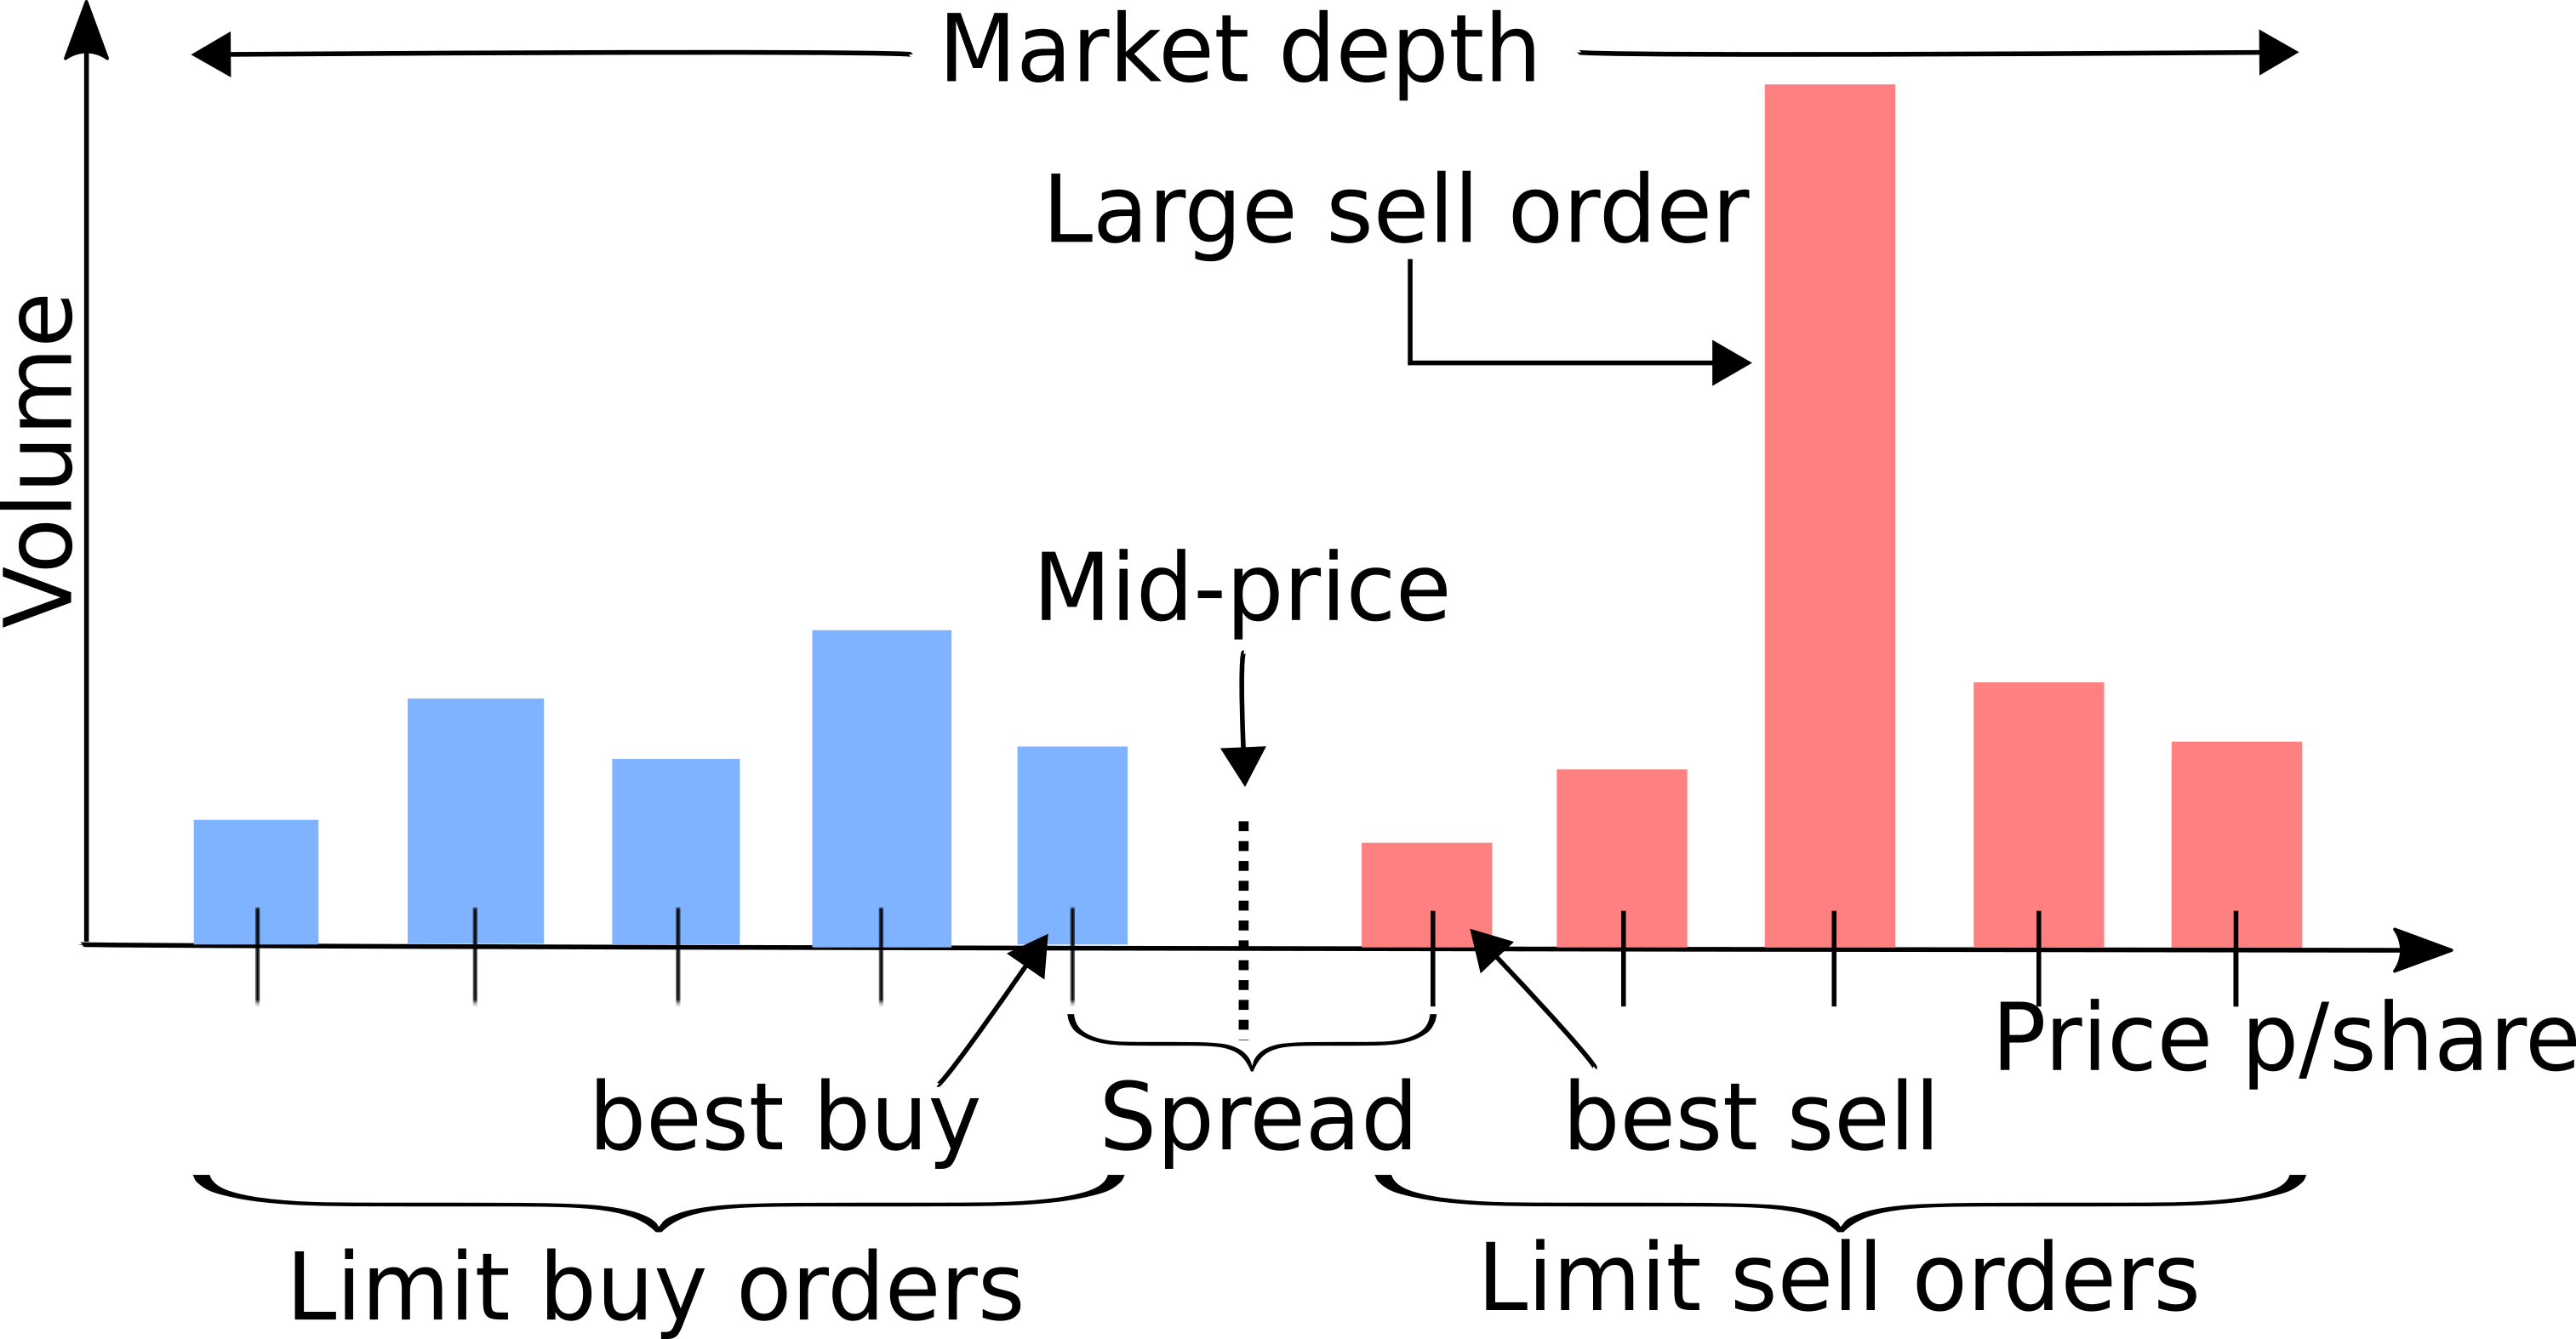
\includegraphics[width=11.5cm, height=7cm]{order_book.png}
\end{frame}

\begin{frame}
\frametitle{Basics of Trading Order Book (TOB)}
\pause
\begin{itemize}[<+->]
\item Buyers/Sellers express their intent to trade by submitting bids/asks
\item These are Limit Orders (LO) with a price $P$ and size $N$
\item Buy LO $(P, N)$ states willingness to buy $N$ shares at a price $\leq P$
\item Sell  LO $(P, N)$ states willingness to sell $N$ shares at a price $\geq P$
\item Trading Order Book aggregates order sizes for each unique price
\item So we can represent with two sorted lists of (Price, Size) pairs
$$\mbox{Bids: } [(P_i^{(b)}, N_i^{(b)}) \mid 1 \leq i \leq m], P_i^{(b)} > P_j^{(b)} \mbox{ for } i < j$$
$$\mbox{Asks: } [(P_i^{(a)}, N_i^{(a)}) \mid 1 \leq i \leq n], P_i^{(a)} < P_j^{(a)} \mbox{ for } i < j$$
\item We call $P_1^{(b)}$ as simply {\em Bid}, $P_1^{(a)}$ as {\em Ask}, $\frac {P_1^{(a)} + P_1^{(b)}} 2$ as {\em Mid}
\item We call $P_1^{(a)} - P_1^{(b)}$ as {\em Spread}, $P_n^{(a)} - P_m^{(b)}$ as {\em Market Depth}
\item A Market Order (MO) states intent to buy/sell $N$ shares at the {\em best possible price(s)} available on the TOB at the time of MO submission
\end{itemize}
\end{frame}

\begin{frame}
\frametitle{Trading Order Book (TOB) Activity}
\pause
\begin{itemize}[<+->]
\item A new Sell LO $(P,N)$ potentially removes best bid prices on the TOB
$$\mbox{Removal: } [(P_i^{(b)}, \min(N_i^{(b)}, \max(0, N - \sum_{j=1}^{i-1} N_j^{(b)}))) \mid (i: P_i^{(b)} \geq P)]$$
\item After this removal, it will add the following to the asks side of the TOB 
$$(P, \max(0, N - \sum_{i: P_i^{(b)} \geq P}  N_i^{(b)}))$$
\item A new Buy MO operates analogously (on the other side of the TOB)
\item A Sell Market Order $N$ will remove the best bid prices on the TOB
$$\mbox{Removal: } [(P_i^{(b)}, \min(N_i^{(b)}, \max(0, N - \sum_{j=1}^{i-1} N_j^{(b)}))) \mid 1 \leq i \leq m]$$
\item A Buy Market Order $N$ will remove the best ask prices on the TOB
$$\mbox{Removal: } [(P_i^{(a)}, \min(N_i^{(a)}, \max(0, N - \sum_{j=1}^{i-1} N_j^{(a)}))) \mid 1 \leq i \leq n]$$
\end{itemize}
\end{frame}

\section{Definition of Optimal Market-Making Problem}

\begin{frame}
\frametitle{TOB Dynamics and Market-Making}
\pause
\begin{itemize}[<+->]
\item Modeling TOB Dynamics involves predicting arrival of MOs and LOs
\item Market-makers are liquidity providers (providers of Buy and Sell LOs)
\item Other market participants are typically liquidity takers (MOs)
\item But there are also other market participants that trade with LOs
\item Complex interplay between market-makers \& other mkt participants
\item Hence, TOB Dynamics tend to be quite complex
\item We view the TOB from the perspective of a single market-make who aims to gain with Buy/Sell LOs of appropriate width/size
\item By anticipating TOB Dynamics \& dynamically adjusting Buy/Sell LOs
\item Goal is to maximize {\em Utility of Gains} at end of a suitable horizon
\item If Buy/Sell LOs are too narrow, more frequent but small gains
\item If Buy/Sell LOs are too wide, less frequent but large gains
\item Market-maker also needs to manage potential unfavorable inventory (long or short) buildup and consequent unfavorable liquidation
\end{itemize}
\end{frame}



\begin{frame}
\frametitle{Notation for Optimal Market-Making Problem}
\pause
\begin{itemize}[<+->]
\item We simplify the setting for ease of exposition
\item Assume finite time steps indexed by $t= 0, 1, \ldots, T$
\item Denote $W_t \in \mathbb{R}$ as Market-maker's wealth at time $t$
\item Denote $I_t \in \mathbb{Z}$ as Market-maker's inventory of shares at time $t$ ($I_0 = 0$)
\item $S_t \in \mathbb{R}^+$ is the TOB Mid Price at time $t$ (assume stochastic process)
\item $P_t^{(b)} \in \mathbb{R}^+, N_t^{(b)} \in \mathbb{Z}^+$ are market maker's Bid Price, Bid Size at time $t$
\item $P_t^{(a)} \in \mathbb{R}^+, N_t^{(a)} \in \mathbb{Z}^+$ are market-maker's Ask Price, Ask Size at time $t$
\item Assume market-maker can add or remove bids/asks costlessly
\item Denote $\delta_t^{(b)} = S_t - P_t^{(b)}$ as Bid Spread, $\delta_t^{(a)} = P_t^{(a)} - S_t$ as Ask Spread
\item Random var $X_t^{(b)} \in \mathbb{Z}_{\geq 0}$ denotes bid-shares ``hit'' {\em up to} time $t$
\item Random var $X_t^{(a)} \in \mathbb{Z}_{\geq 0}$ denotes ask-shares ``lifted'' {\em up to} time $t$
$$W_{t+1} = W_t + P_t^{(a)} \cdot (X_{t+1}^{(a)} - X_t^{(a)}) - P_t^{(b)} \cdot (X_{t+1}^{(b)} - X_t^{(b)}) \mbox{ , } I_t = X_t^{(b)} - X_t^{(a)}$$
\item Goal to maximize $E[U(W_T + I_T \cdot S_T)]$ for appropriate concave $U(\cdot)$
\end{itemize}
\end{frame}

\begin{frame}
\frametitle{Markov Decision Process (MDP) Formulation}
\pause
\begin{itemize}[<+->]
\item Order of MDP activity in each time step $0 \leq t \leq T-1$:
\begin{itemize}
\item Observe {\em State} $:= (t, S_t, W_t, I_t)$
\item Perform {\em Action} $:= (P_t^{(b)}, N_t^{(b)}, P_t^{(a)}, N_t^{(a)})$
\item Experience TOB Dynamics resulting in:
\begin{itemize}
\item random bid-shares hit $=X_{t+1}^{(b)} - X_t^{(b)}$ and ask-shares lifted $=X_{t+1}^{(a)} - X_t^{(a)}$
\item update of $W_t$ to $W_{t+1}$, update of $I_t$ to $I_{t+1}$
\item stochastic evolution of $S_t$ to $S_{t+1}$
\end{itemize}
\item Receive next-step ($t+1$) {\em Reward} $R_{t+1}$
$$
R_{t+1} :=
\begin{cases}
0 & \text{ for }1 \leq t+1 \leq T-1 \\
U(W_{t+1} + I_{t+1} \cdot S_{t+1}) & \text{ for } t+1 = T \\
\end{cases}
$$
\end{itemize}
\item Goal is to find an {\em Optimal Policy} $\pi^*$:
$$\pi^*(t, S_t, W_t, I_t) = (P_t^{(b)}, N_t^{(b)}, P_t^{(a)}, N_t^{(a)}) \mbox{ that maximizes } \mathbb{E}[\sum_{t=1}^T R_t]$$
\item Note: Discount Factor when aggregating Rewards in the MDP is 1
\end{itemize}
\end{frame}

\section{Derivation of Avellaneda-Stoikov Analytical Solution}
\begin{frame}
\frametitle{Avellaneda-Stoikov Continuous Time Formulation}
\pause
\begin{itemize}[<+->]
\item We go over the \href{https://www.math.nyu.edu/faculty/avellane/HighFrequencyTrading.pdf}{\underline{\textcolor{blue}{landmark paper by Avellaneda and Stoikov in 2006}}}
\item They derive a simple, clean and intuitive analytical solution
\item We adapt our discrete-time notation to their continuous-time setting
\item $X_t^{(b)}, X_t^{(a)}$ are {\em Poisson processes} with {\em arrival-rate} means $\lambda_t^{(b)}, \lambda_t^{(a)}$
$$dX_t^{(b)} \sim Poisson(\lambda_t^{(b)} \cdot dt) \mbox{ , } dX_t^{(a)} \sim Poisson(\lambda_t^{(a)} \cdot dt)$$
$$\lambda_t^{(b)} = f^{(b)}(\delta_t^{(b)}) \mbox{ , } \lambda_t^{(a)} = f^{(a)}(\delta_t^{(a)}) \mbox{ for decreasing functions } f^{(b)}, f^{(a)}$$
$$dW_t = P_t^{(a)} \cdot dX_t^{(a)} - P_t^{(b)} \cdot dX_t^{(b)} \mbox{ , } I_t = X_t^{(b)} - X_t^{(a)} \mbox{ (note: } I_0 = 0 \mbox{)}$$
\item Since infinitesimal Poisson random variables $dX_t^{(b)}$ (shares hit in time $dt$) and $dX_t^{(a)}$ (shares lifted in time $dt$) have zero probability mass for values greater than 1, choices of $N_t^{(b)}$ and $N_t^{(a)}$ are irrelevant
\item This simplifies the {\em Action} at time $t$ to be just the pair: $(\delta_t^{(b)}, \delta_t^{(a)})$
\item TOB Mid Price Dynamics: $dS_t = \sigma \cdot dz_t$ (scaled brownian motion)
\item Utility function $U(x) = -e^{-\gamma x}$ where $\gamma$ is coefficient of risk-aversion  
\end{itemize}
\end{frame}

\section{Real-world Optimal Market-Making and Reinforcement Learning}

\begin{frame}
\frametitle{Real-world Market-Making and Reinforcement Learning}
\pause
\begin{itemize}[<+->]
\item Arbitrary Price Dynamics $f_t(\cdot)$ and Temporary Price Impact $g_t(\cdot)$
\item Non-stationarity/non-linear dynamics/impact require (Numerical) DP
\item Frictions: Discrete Prices/Sizes, Constraints on Prices/Sizes, Fees
\item Large State space incorporate various external factors in the State
\item We could also represent the entire TOB within the State
\item So then we'd have to develop a simulator capturing all of the above
\item Simulator is a {\em Data-learnt Sampling Model} of TOB Dynamics 
\item In practice, we'd need to also capture {\em Cross-Asset Market Impact}
\item Using this simulator and neural-networks func approx, we can do RL
\item References: \href{https://www.cis.upenn.edu/~mkearns/papers/rlexec.pdf}{\underline{\textcolor{blue}{Nevmyvaka, Feng, Kearns; 2006}}} and \href{https://arxiv.org/pdf/1906.02312.pdf}{\underline{\textcolor{blue}{Vyetrenko, Xu; 2019}}}
\item Exciting area for Future Research as well as Engineering Design
\end{itemize}
\end{frame}

\end{document}
